% This work is made available under the terms of the
% Creative Commons Attribution-ShareAlike 4.0 license,
% http://creativecommons.org/licenses/by-sa/4.0/.
%
% Version: $Revision$

\documentclass[a4paper]{book}

\usepackage{wrapfig}
\usepackage{graphicx}
\usepackage{hyperref}
\usepackage{multirow}
\usepackage{scalefnt}
\usepackage{tikz}
\usepackage{varwidth}

% watermark -- for draft stage
\usepackage[firstpage]{draftwatermark}
\SetWatermarkLightness{0.9}
\SetWatermarkScale{5}

% Copyright (c) 2009 by the University of Waikato, Hamilton, NZ. 
% This work is made available under the terms of the 
% Creative Commons Attribution-ShareAlike 3.0 license, 
% http://creativecommons.org/licenses/by-sa/3.0/. 
%
% Version: $Revision$

\newenvironment{tight_itemize}{
\begin{itemize}
  \setlength{\itemsep}{1pt}
  \setlength{\parskip}{0pt}
  \setlength{\parsep}{0pt}}{\end{itemize}
}

\newenvironment{tight_enumerate}{
\begin{enumerate}
  \setlength{\itemsep}{1pt}
  \setlength{\parskip}{0pt}
  \setlength{\parsep}{0pt}}{\end{enumerate}
}

% if you just need a simple heading
% Usage:
%   \heading{the text of the heading}
\newcommand{\heading}[1]{
  \vspace{0.3cm} \noindent \textbf{#1} \newline
}

\newcommand{\icon}[1]{\tikz[baseline=-3pt]\node[inner sep=0pt,outer sep=0pt]{\includegraphics[height=1.1em]{#1}};}


\title{
  \textbf{ADAMS} \\
  {\Large \textbf{A}dvanced \textbf{D}ata mining \textbf{A}nd \textbf{M}achine
  learning \textbf{S}ystem} \\
  {\Large Module: adams-spreadsheet} \\
  \vspace{1cm}
  
\includegraphics[width=2cm]{images/spreadsheet-module.png} \\
}
\author{
  Peter Reutemann
}

\setcounter{secnumdepth}{3}
\setcounter{tocdepth}{3}

\begin{document}

\begin{titlepage}
\maketitle

\thispagestyle{empty}
\center
\begin{table}[b]
	\begin{tabular}{c l l}
		\parbox[c][2cm]{2cm}{\copyright 2012-2017} &
		\parbox[c][2cm]{5cm}{
\includegraphics[width=5cm]{images/coat_of_arms.pdf}} \\
	\end{tabular}
	
\includegraphics[width=12cm]{images/cc.png} \\
\end{table}

\end{titlepage}

\tableofcontents
\listoffigures
%\listoftables


%%%%%%%%%%%%%%%%%%%%%%%%%%%%%%%%%%%
\chapter{Introduction}
Tabular data is a very common data format, not only for machine learning.
The \textit{spreadsheet} module offers some basic spreadsheet support for
reading/writing and some generic actors. Other modules, like the \textit{odf}
or \textit{excel} one, offer other native readers and writers. The data
read by these readers can be processed with the same actors.


%%%%%%%%%%%%%%%%%%%%%%%%%%%%%%%%%%%
\chapter{Flow}
A lot of the following actors and conversion schemes offer either an index of
a column or a range of columns as a parameter. In addition to the usual
\textit{first/last/\ldots} placeholders, you can use the actual column names
(case-insensitive). This makes an actor less error-prone, in case the order 
of the columns may change.

The following standalones are available:
\begin{tight_itemize}
	\item \textit{LookUpInit} -- Initializes an empty lookup table in
	storage, which needs populating using the \textit{LookUpAdd}
	transformer.\footnote{adams-spreadsheet-lookup2.flow}
\end{tight_itemize}
The following sources are available:
\begin{tight_itemize}
	\item \textit{DatabaseMetaData} -- outputs spreadsheets with information
	obtained from the meta-data of a database connection.
	\item \textit{NewSpreadSheet} -- for creating an empty spreadsheet with
	pre-defined columns.
	\item \textit{SpreadSheetDbReader} -- turns results from SQL queries into
	spreadsheet objects.\footnote{adams-spreadsheet-database\_access.flow}
	\item \textit{LookUp} -- Outputs a value from a stored lookup table,
	identified by a user-supplied key.\footnote{adams-spreadsheet-lookup.flow}
	\item \textit{LookUpTable} -- Outputs a stored lookup table as
	spreadsheet.\footnote{adams-spreadsheet-lookup.flow}
\end{tight_itemize}
The following transformers are available:
\begin{tight_itemize}
	\item \textit{LookUp} -- obtains the value associated with the string 
	received as input from an internally stored lookup 
	table.\footnote{adams-spreadsheet-lookup.flow}
	\item \textit{LookUpAdd} -- adds a key/value pair to a lookup 
	table.\footnote{adams-spreadsheet-lookup.flow}
	\item \textit{LookUpInit} -- initializes a lookup table by using two columns
	from a spreadsheet, one acting as key, the other as 
	value.\footnote{adams-spreadsheet-lookup.flow}
	\item \textit{LookUpRemove} -- removes a key/value pair from a lookup 
	table.\footnote{adams-spreadsheet-lookup.flow}
	\item \textit{SpreadSheetAggregate} -- aggregates rows in a spreadsheet
	(min, max, average, standard deviation, etc).\footnote{adams-spreadsheet-aggregate.flow}
	\item \textit{SpreadSheetAnonymize} -- for anonymizing 
	columns.\footnote{adams-spreadsheet-anonymize\_columns.flow}
	\item \textit{SpreadSheetCellFinder} -- outputs row/column pairs of
	cells that matched the specified criteria of the cell finder algorithm.
	\item \textit{SpreadSheetCollapse} -- collapses cell values of rows with
	the same key into single cell.
	\item \textit{SpreadSheetColumnFilter} -- filters columns using a column
	finder scheme.\footnote{adams-spreadsheet-filter\_columns.flow}
	\item \textit{SpreadSheetColumnIterator} -- iterates over all the columns
	in the spreadsheet and outputs the names.\footnote{adams-spreadsheet-iterate\_cols.flow}
	\item \textit{SpreadSheetColumnStatistic} -- generates statistics for a 
	spreadsheet column.\footnote{adams-spreadsheet-column\_statistics.flow}
	\item \textit{SpreadSheetColumnsByName} -- generates a new spreadsheet with
	only the columns that match a regular expression (inverting is possible as well).
	\item \textit{SpreadSheetCommonIDs} -- determines common (or not in common)
	IDs from two or more spreadsheets.
	\item \textit{SpreadSheetConvertCells} -- applies arbitrary conversion
	schemes to individual cells.
	\item \textit{SpreadSheetConvertHeaderCells} -- applies arbitrary conversion 
	schemes to the header cells.
	\item \textit{SpreadSheetCopyColumns} -- copies the content of a range of
	columns into new columns.
	\item \textit{SpreadSheetCopyRows} -- duplicates the content of a range of
	rows at another location in the spreadsheet.\footnote{adams-spreadsheet-copy\_rows.flow}
	\item \textit{SpreadSheetDifference} -- computes the difference between two
	spreadsheets.
	\item \textit{SpreadSheetExtractArray} -- allows the extraction of a
	row or column from a spreadsheet.
	\item \textit{SpreadSheetFileReader} -- for reading spreadsheet
	files; depending on the reader, multiple sheets can get read at 
	once.\footnote{adams-spreadsheet-output\_cells.flow}
	\item \textit{SpreadSheetFilter} -- applies the specified filter to the
	spreadsheet.
	\item \textit{SpreadSheetGetCell} -- retrieves the value of a specific cell
	in the spreadsheet.\footnote{adams-spreadsheet-output\_cells.flow}
	\item \textit{SpreadSheetGetColumnIndex} -- retrieves the 1-based index columns
	which name matches a regular expression.\footnote{adams-spreadsheet-get\_column\_index.flow}
	\item \textit{SpreadSheetGetHeaderCell} -- retrieves the value of a specific cell
	in the header row of a spreadsheet.
	\item \textit{SpreadSheetHistogramRanges} -- outputs the ranges generated by the
	ArrayHistogram statistic.
	\item \textit{SpreadSheetInfo} -- generates basic information on the
	spreadsheet object.
	\item \textit{SpreadSheetInsertColumn} -- inserts a column in the spreadsheet,
	initializes the cells with a user-defined value.
	\item \textit{SpreadSheetInsertRow} -- inserts a row in the spreadsheet,
	initializes the cells with a user-defined value.
	\item \textit{SpreadSheetInsertRowScore} -- inserts a column in the spreadsheet,
	containing a score calculate for the corresponding row.
	\item \textit{SpreadSheetMatrixStatistic} -- calculates statistics from
	the whole spreadsheet (or a defined subset).
	\item \textit{SpreadSheetMerge} -- merges multiple spreadsheets into a single
	one.\footnote{adams-spreadsheet-simple\_merge.flow, adams-spreadsheet-merge\_using\_id.flow}
	\item \textit{SpreadSheetPlotGenerator} -- turns a spreadsheet into plot
	containers to be displayed in the \textit{SequencePlotter} 
	sink.\footnote{adams-spreadsheet-spreadsheet\_plot1.flow, 
	adams-spreadsheet-spreadsheet\_plot2.flow, adams-spreadsheet-statistic.flow}
	\item \textit{SpreadSheetQuery} -- allows to run an SQL-like query on a 
	spreadsheet to select a subset of rows/columns, delete rows, rename columns, 
	update cells.\footnote{adams-spreadsheet-query.flow, adams-spreadsheet-date\_queries.flow, 
	adams-spreadsheet-celltype\_queries.flow}
	\item \textit{SpreadSheetRemoveColumn} -- removes columns from a spreadsheet.
	\item \textit{SpreadSheetRemoveRow} -- removes rows from a spreadsheet.
	\item \textit{SpreadSheetReorderColumns} -- reorders columns in a spreadsheet, 
	also allows duplicating/dropping of columns.
	\item \textit{SpreadSheetReplaceCellValue} -- replaces cell values that
	match a regular expression.
	\item \textit{SpreadSheetRowBuffer} -- buffers incoming row objects and
	outputs spreadshets or outputs single rows when receiving spreadsheets.
	\item \textit{SpreadSheetRowFilter} -- filters rows using a row
	finder scheme.\footnote{adams-spreadsheet-filter\_rows.flow}
	\item \textit{SpreadSheetRowStatistic} -- generates statistics for a 
	spreadsheet row.\footnote{adams-spreadsheet-row\_statistics.flow}
	\item \textit{SpreadSheetSelectSubset} -- allows the user to select a
	subset from a spreadsheet.
	\item \textit{SpreadSheetSetCell} -- sets the value of a specific cell
	in the spreadsheet.\footnote{adams-spreadsheet-set\_cells.flow}
	\item \textit{SpreadSheetSetHeaderCell} -- sets the value of a specific cell
	in the header row of a spreadsheet.
	\item \textit{SpreadSheetSort} -- sorts the rows a spreadsheet using an arbitrary
	number of columns (ascending or descending).
	\item \textit{SpreadSheetSortColumns} -- sorts the columns (or a subset of
	columns) of a spreadsheet using a specified comparator.
	\item \textit{SpreadSheetStatistic} -- calculates statistics using the
	data stored in the spreadsheet.\footnote{adams-spreadsheet-statistic.flow}
	\item \textit{SpreadSheetSubset} -- for obtaining a subset of the 
	spreadsheet object (subset of columns and/or rows).
	\item \textit{SpreadSheetSubsetByValue} -- splits a spreadsheet into 
	subsets using the unique (string) values in a column for grouping.
	\item \textit{SpreadSheetStorageRowIterator} -- iterates over a range of 
	rows/columns and stores the cell values in internal storage.
	\item \textit{SpreadSheetTransformCells} -- applies an arbitrary callable
	transformer to individual cells.
	\item \textit{SpreadSheetTransformHeaderCells} -- applies an arbitrary callable
	transformer to the header cells.
	\item \textit{SpreadSheetVariableRowIterator} -- iterates over a range of 
	rows/columns and stores the cell values in 
	variables.\footnote{adams-spreadsheet-variable\_row\_iterator.flow}
\end{tight_itemize}
The following sinks are available:
\begin{tight_itemize}
	\item \textit{JFreeChartFileWriter} -- generates plots from spreadsheet
	columns using JFreeChart\cite{jfreechart} and writes them to disk.
	\item \textit{JFreeChartPlot} -- allows plotting of columns from
	spreadsheets using JFreeChart\cite{jfreechart}.
	\item \textit{SpreadSheetDbWriter} -- for storing a spreadsheet in a
	database.\footnote{adams-spreadsheet-database\_access.flow}
	\item \textit{SpreadSheetDisplay} -- for displaying spreadsheet objects
	in tabular form.\footnote{adams-spreadsheet-display.flow}
	\item \textit{SpreadSheetFileWriter} -- writes spreadsheet objects to a file
	with the chosen writer class; depending on the writer either a single or
	multiple sheets can get written at once.
	\item \textit{SpreadSheetRowViewer} -- displays the numeric values of
	rows from a spreadsheet as line plots.
\end{tight_itemize}
The following boolean conditions are available:
\begin{tight_itemize}
	\item \textit{HasColumn} -- checks whether the spreadsheet passing through
	has a column with that name.
\end{tight_itemize}
The following conversion schemes are available:
\begin{tight_itemize}
	\item \textit{ContainerToSpreadSheet} -- for converting any flow container 
	(e.g., a prediction container) into a spreadsheet for better visualization.
	\item \textit{ConvertSpreadSheetRows} -- converts the data rows in a spreadsheet
	into a different format, e.g., into sparse representation.
	\item \textit{DoubleMatrixToSpreadSheet} -- converts a two-dimensional double
	array (i.e., matrix) into a spreadsheet object.
	\item \textit{MapToSpreadSheet} -- turns a \textit{java.util.Map} object
	into a spreadsheet.
	\item \textit{NotesToSpreadSheet} -- generates a spreadsheet from a Notes
	object.
	\item \textit{PropertiesToSpreadSheet} -- generates a spreadsheet from a 
	Properties object.
	\item \textit{RenameSpreadSheet} -- renames a spreadsheet.
	\item \textit{RenameSpreadSheetColumn} -- renames a single column in a 
	spreadsheet.
	\item \textit{ReportToSpreadSheet} -- generates a spreadsheet from a
	Report object.
	\item \textit{SpreadSheetAddFormulaColumn} -- adds a column with a row-wise,
	user-supplied formula.
	\item \textit{SpreadSheetAddFormulaRow} -- adds a row with a column-wise,  
	user-supplied formula.
	\item \textit{SpreadSheetAddRowID} -- adds an ID column to the spreadsheet
	that contains the row index as value
	\item \textit{SpreadSheetAddSumColumn} -- adds a column with a row-wise sum 
	formula.
	\item \textit{SpreadSheetAddSumRow} -- adds a row with a column-wise sum 
	formula.
	\item \textit{SpreadSheetAnyColumnToString} -- converts any data types in 
	a column to strings.
	\item \textit{SpreadSheetCellLocationToCoordinates} -- turns a cell location
	into an integer array of 1-based coordinates
	\item \textit{SpreadSheetCellLocationToPosition} -- turns a cell location
	obtained from a cell finder into a position string (eg 'A2').
	\item \textit{SpreadSheetColumnFinderToRange} -- outputs a range string
	of the columns that the finder located (eg '1-6,8').
	\item \textit{SpreadSheetDoubleColumnToLong} -- converts any floating values
	to integer (= long) values.
	\item \textit{SpreadSheetDoubleColumnToString} -- converts any floating values
	to strings.
	\item \textit{SpreadSheetEscapeColumnName} -- ensures that a column is escaped
	correctly in order to be used in column range expressions.
	\item \textit{SpreadSheetInsertCellLocation} -- replaces a placeholder in 
	a string with a cell location (e.g., ``A1'').
	\item \textit{SpreadSheetInsertColumnPosition} -- replaces a placeholder in
	a string with a column position (e.g., ``BG``)
	\item \textit{SpreadSheetJoinColumns} -- joins two or more columns in
	a spreadsheet into a single one.
	\item \textit{SpreadSheetLongColumnToDouble} -- converts long values in a
	column to double objects.
	\item \textit{SpreadSheetMaterializeFormulas} -- replaces formulas in cells
	with the current value of the formula.
	\item \textit{SpreadSheetRowFinderToRange} -- outputs a range string
	of the rows that the finder located (eg '1-6,8').
	\item \textit{SpreadSheetStringSplitColumn} -- splits the string representation 
	of a column into multiple columns using a regular expression.
	\item \textit{SpreadSheetStringColumnToBoolean} -- converts strings values in a 
	column to boolean objects.
	\item \textit{SpreadSheetStringColumnToDate} -- converts strings values in a 
	column to date objects.
	\item \textit{SpreadSheetStringColumnToDateTime} -- converts strings values in a 
	column to date/time objects.
	\item \textit{SpreadSheetStringColumnToDouble} -- converts strings values in a 
	column to floating values.
	\item \textit{SpreadSheetStringColumnToLong} -- converts strings values in a 
	column to integer (= long) values.
	\item \textit{SpreadSheetStringColumnToTime} -- converts strings values in a 
	column to time objects.
	\item \textit{SpreadSheetToCreateTableStatement} -- turns a spreadsheet with
	SQL column names and types into a SQL 'CREATE TABLE' statement.
	\item \textit{SpreadSheetToDoubleMatrix} -- turns all the numeric columns of
	a spreadsheet into a two-dimensional double matrix.
	\item \textit{SpreadSheetToJson} -- turns a spreadsheet into a JSON array object.
	\item \textit{SpreadSheetToMap} -- uses two columns from a spreadsheet
	(key and value) to populate a \textit{java.util.Map} object.
	\item \textit{SpreadSheetToNumeric} -- turns all non-numeric cells into numeric
	ones; can replace missing values as well.
	\item \textit{SpreadSheetToStringMatrix} -- turns all columns of
	a spreadsheet into a two-dimensional string matrix.
	\item \textit{SpreadSheetUnescapeColumnName} -- reverses the escaping for
	a column name.
	\item \textit{SpreadSheetUniqueColumnNames} -- ensures that the column
	names uniquely identify a column.
	\item \textit{StringToSpreadSheet} -- parses a string in CSV format and
	turns it into a spreadsheet object.
	\item \textit{StringMatrixToSpreadSheet} -- turns a (two-dimensional) 
	string matrix into a spreadsheet.
	\item \textit{TransposeSpreadSheet} -- swaps columns with rows.
\end{tight_itemize}

%%%%%%%%%%%%%%%%%%%%%%%%%%%%%%%%%%%
\chapter{Tools}
The \textit{Spreadsheet file viewer} is a simple tool for loading all spreadsheet
file formats that ADAMS supports. Despite its name, the tool also allows you to
modify cell values and save them back to a file. Figure \ref{spreadsheet-viewer} shows a
dataset that was loaded from a CSV (comma-separated values) file.

\begin{figure}[htb]
  \centering
  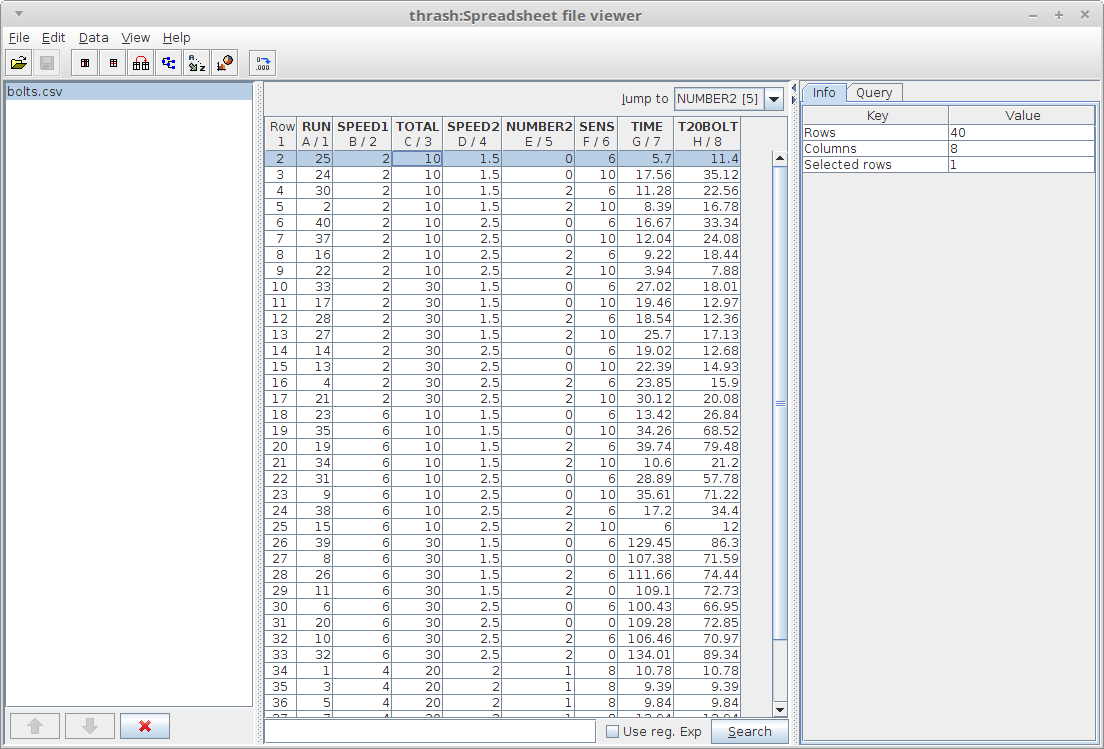
\includegraphics[width=10.0cm]{images/spreadsheet-viewer.png}
  \caption{Viewer for spreadsheet files.}
  \label{spreadsheet-viewer}
\end{figure}

If there are more spreadsheet file formats registered, you can save the
currently displayed spreadsheet in another format. Printing, of course, is
available throught the \textit{Send to} menu. By default, the viewer displays
each cell with as many digits after the decimal point as necessary. But you can
also unify this and specify how many digits should be used for all floating
point cells.

\clearpage
\section{Filtering and processing}
The viewer supports some basic filtering and processing:
\begin{tight_itemize}
	\item \textit{columns} -- creates a subset of the spreadsheet by selecting
	a subset of columns, e.g., all columns which name starts with a certain string.
	\item \textit{rows} -- creates a subset of the spreadsheet by selecting
	a subset of rows, e.g., rows with a certain value in a column.
	\item \textit{convert} -- applies a conversion scheme specific to 
	spreadsheets, e.g., transposing a spreadsheet.
	\item \textit{transform} -- applies a flow transformer specific to 
	spreadsheets, e.g., inserting a column or creating a subset.
\end{tight_itemize}
Figures \ref{spreadsheet-viewer-rowfilter_setup} and \ref{spreadsheet-viewer-rowfilter_result}
show the setup for a row finder filter and the resulting new spreadsheet.

\begin{figure}[ht]
  \begin{minipage}[t]{0.4\linewidth}
    \centering
    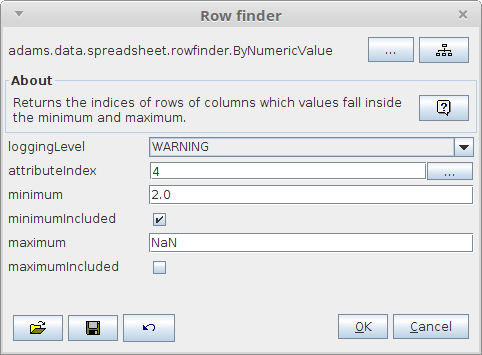
\includegraphics[width=4.0cm]{images/spreadsheet-viewer-rowfilter_setup.png}
    \caption{Row finder setup.}
    \label{spreadsheet-viewer-rowfilter_setup}
  \end{minipage}
  \hspace{0.5cm}
  \begin{minipage}[t]{0.6\linewidth}
    \centering
    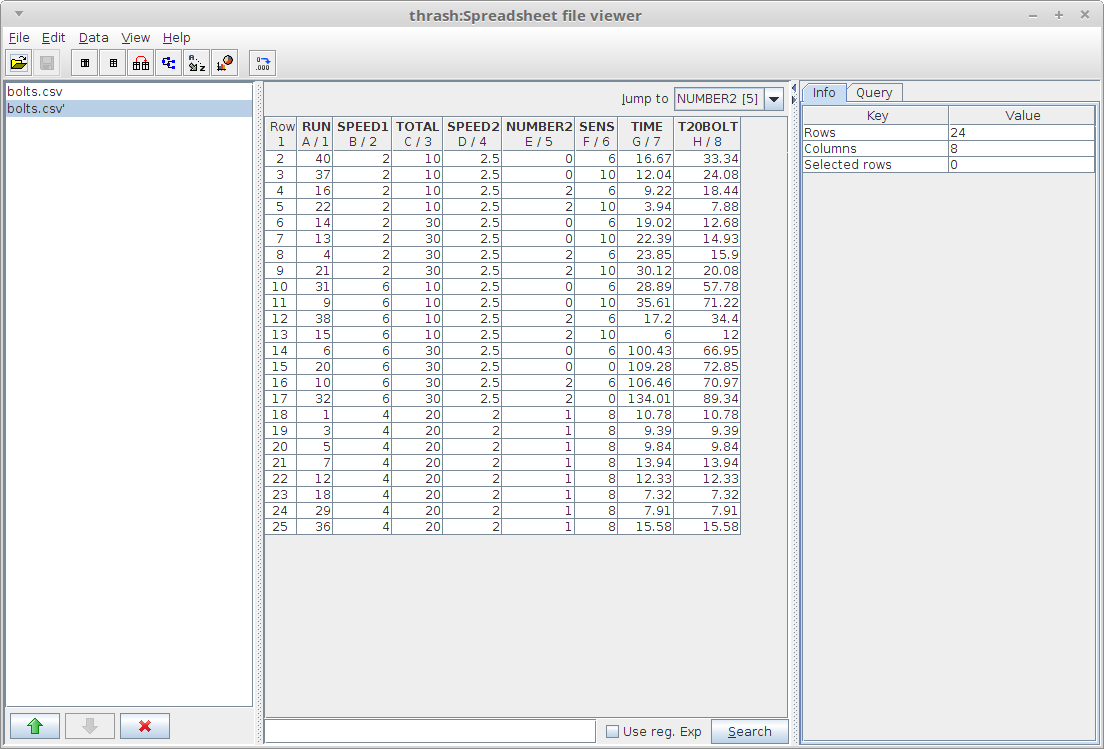
\includegraphics[width=7.0cm]{images/spreadsheet-viewer-rowfilter_result.png}
    \caption{The filtered spreadsheet.}
    \label{spreadsheet-viewer-rowfilter_result}
  \end{minipage}
\end{figure}

\section{Plug-ins}
The viewer can be extended with two sorts of plug-ins:
\begin{tight_itemize}
	\item ones that generate a view based on the current sheet (``view'')
	\item ones that process the current sheet (``data'')
\end{tight_itemize}

\subsection{View plug-ins}
A view plug-in is derived from the following super-class:
\begin{verbatim}
  adams.gui.tools.spreadsheetviewer.AbstractViewPlugin
\end{verbatim}
There are three methods that need implementing:
\begin{tight_itemize}
	\item \textit{getMenuText()} -- returns the text used for the menu item 
	and the title of the dialog displaying the generated view.
	\item \textit{getMenuIcon()} -- returns the name of the icon (no path)
	that should be displayed in the menu (use null to display no icon). 
	\item \textit{doGenerate(SpreadSheet)} -- this method generates the
	actual view in form of a \textit{adams.gui.core.BasePanel}.
\end{tight_itemize}
An example is the \textit{Statistics} plug-in, which shows simple statistics
for a spreadsheet, number of rows and colums and what types of columns
are present:
\begin{verbatim}
  adams.gui.tools.spreadsheetviewer.Statistics
\end{verbatim}
Further superclasses:
\begin{tight_itemize}
	\item \textit{AbstractSelectedSheetsViewPlugin} -- for view plugins that
	operate on one or more spreadsheets that the user selects.
	\item \textit{AbstractSelectedSheetsViewPluginWithGOE} -- same as
	\textit{AbstractSelectedSheetsViewPlugin} but offers the user to change
	the settings through a GenericObjectEditor view.
\end{tight_itemize}

\subsection{Data plug-ins}
A view plug-in is derived from the following super-class:
\begin{verbatim}
  adams.gui.tools.spreadsheetviewer.AbstractDataPlugin
\end{verbatim}
There are four methods that need implementing:
\begin{tight_itemize}
	\item \textit{getMenuText()} -- returns the text used for the menu item 
	and the title of the dialog displaying the generated view.
	\item \textit{getMenuIcon()} -- returns the name of the icon (no path)
	that should be displayed in the menu (use null to display no icon). 
	\item \textit{doProcess(SpreadSheet)} -- this method processes the
	current spreadsheet and returns a new spreadsheet object.
	\item \textit{isInPlace()} -- returns whether the generated spreadsheet
	object should simply replace the current one (``in-place'') or added as
	new tab.
\end{tight_itemize}
Further superclasses:
\begin{tight_itemize}
	\item \textit{AbstractSelectedSheetsDataPlugin} -- for data plugins that
	operate on one or more spreadsheets that the user selects (see 
	\textit{Append} plugin).
	\item \textit{AbstractSelectedSheetsDataPluginWithGOE} -- same as
	\textit{AbstractSelectedSheetsDataPlugin} but offers the user to change
	the settings through a GenericObjectEditor view (see \textit{Merge} plugin).
\end{tight_itemize}

%%%%%%%%%%%%%%%%%%%%%%%%%%%%%%%%%%%
\clearpage
\chapter{Formulas}
ADAMS supports formulas with a range of basic functions. The following lists
describe briefly what functionality is available. A full list is available 
through the \textit{Help -> Formulas} menu in the \textit{Spreadsheet file viewer}. \\

\noindent Operands:
\begin{tight_itemize}
	\item \textit{$NUM + NUM$} -- addition
	\item \textit{$NUM - NUM$} -- subtraction
	\item \textit{$NUM * NUM$} -- multiplication
	\item \textit{$NUM / NUM$} -- division
	\item \textit{$NUM \wedge NUM$} -- exponential
	\item \textit{$NUM \% NUM$} -- modulo
\end{tight_itemize}

\noindent Boolean operations:
\begin{tight_itemize}
	\item \textit{$<$} -- less than
	\item \textit{$<=$} -- less than or equal
	\item \textit{$>$} -- greater than
	\item \textit{$>=$} -- greater than or equal
	\item \textit{$=$} -- equals
	\item \textit{$!=$} -- does not equal (alternative: \textit{$<>$})
	\item \textit{$!$} -- negation
	\item \textit{$\&$} -- and
	\item \textit{$|$} -- or
\end{tight_itemize}

\noindent Numeric functions:
\begin{tight_itemize}
	\item \textit{abs} -- absolute value of a cell/number.
	\item \textit{average} -- average computed from a range of cells.
	\item \textit{ceil} -- smallest value that is greater than or equal to the cell/number and is equal to a mathematical integer.
	\item \textit{cos} -- the trigonometric cosine of a number/cell.
	\item \textit{countblank} -- counts empty/missing value cells in a range of cells.
	\item \textit{countif} -- counts value only a condition is true.
	\item \textit{exp} -- Euler's number e raised to the power of a number/cell.
	\item \textit{floor} -- largest value that is less than or equal to the cell/number and is equal to a mathematical integer.
	\item \textit{if[else]} -- if-then-else construct.
	\item \textit{intercept} -- compute the intercept of linear regression between two cell ranges.
	\item \textit{log} -- natural logarithm (base e) of a number/cell.
	\item \textit{max} -- largest value from range of cells.
	\item \textit{min} -- smallest value from range of cells.
	\item \textit{pow[er]} -- the first number/cell raised to the power of the second number/cell.
	\item \textit{rint} -- returns number that is closest in value to the number/cell and is equal to a mathematical integer.
	\item \textit{sin} -- trigonometric sine of a number/cell.
	\item \textit{slope} -- compute the slope of linear regression between two cell ranges.
	\item \textit{sqrt} -- the correctly rounded positive square root of a number/cell.
	\item \textit{stdev} -- the sample standard deviation from a range of cells.
	\item \textit{stdevp} -- the population standard deviation from a range of cells.
	\item \textit{sum} -- the sum over a range of cells.
	\item \textit{sumif} -- the conditional sum over a range of cells.
	\item \textit{tan} -- trigonometric tangent of a number/cell.
\end{tight_itemize}

\noindent String functions:
\begin{tight_itemize}
	\item \textit{concatenate} -- concatenates up to 5 strings.
	\item \textit{find} -- returns the location of a search string in a string.
	\item \textit{left} -- returns substring of specified length from the left of the string.
	\item \textit{len[gth]} -- the length of a string.
	\item \textit{lower[case]} -- converts string to a lowercase one.
	\item \textit{matches} -- matches a string against a regular expression.
	\item \textit{mid} -- returns substring of specified length from the specified positiojn in the string.
	\item \textit{right} -- returns substring of specified length from the right of the string.
	\item \textit{replace} -- replaces a substring at a specified position with a new string.
	\item \textit{rept} -- returns a string made up of X copies of the supplied string.
	\item \textit{trim} -- removes all leading and trailing whitespaces.
	\item \textit{substr} -- creates a substring from a string, given start/end position.
	\item \textit{substiture} -- replaces occurrences of a search string in a string with a new string.
	\item \textit{upper[case]} -- converts string to an uppercase one.
\end{tight_itemize}

\noindent Date/time functions:
\begin{tight_itemize}
	\item \textit{year} -- extracts the year from a date/time cell.
	\item \textit{month} -- extracts the month from a date/time cell.
	\item \textit{day} -- extracts the day from a date/time cell.
	\item \textit{hour} -- extracts the hour from a date/time cell.
	\item \textit{minute} -- extracts the minute from a date/time cell.
	\item \textit{second} -- extracts the second from a date/time cell.
	\item \textit{weekday} -- extracts the weekday from a date/time cell (Sunday=1, Saturday=7).
	\item \textit{weeknum} -- extracts the week number from a date/time cell.
\end{tight_itemize}

%%%%%%%%%%%%%%%%%%%%%%%%%%%%%%%%%%%
\clearpage
\chapter{Troubleshooting}
\section{Fractional times}
Despite database systems supporting fractional times, i.e., times with
fractional seconds (= milliseconds), the JDBC interface does not support
this (at this stage). This results in fractions always getting set to 0.

However, JDBC drivers, like the MySQL one starting with 5.1.37, may support
in some cases the sending of fractional seconds to the server where the may
be subject to rounding (for MySQL use \texttt{sendFractionalSeconds=true|false}
in the JDBC URL).

In order to avoid the truncating of fractions, you can do two things:
\begin{tight_itemize}
  \item Create your own queries and have them executed using the \textit{ExecSQL}
  standalone - this bypasses the JDBC driver's checks for fractions.
  \item Turn the columns in the spreadsheet, when using the \textit{SpreadSheetDbWriter},
  into strings. They will get converted automatically, at least in the case
  of MySQL, automatically into fractional times again before being inserted.
  Either use the \textit{SpreadSheetAnyColumnToString} conversion or
  use \texttt{concat("", column\_name)} to return the column \textit{column\_name}
  as string from the database in the first place.
\end{tight_itemize}

%%%%%%%%%%%%%%%%%%%%%%%%%%%%%%%%%%%
% Copyright (c) 2009-2012 by the University of Waikato, Hamilton, NZ. 
% This work is made available under the terms of the 
% Creative Commons Attribution-ShareAlike 4.0 license,
% http://creativecommons.org/licenses/by-sa/4.0/.
%
% Version: $Revision$

\begin{thebibliography}{999}
	% to make the bibliography appear in the TOC
	\addcontentsline{toc}{chapter}{Bibliography}

    % references
	\bibitem{adams}
		\textit{ADAMS} -- Advanced Data mining and Machine learning System \\
		\url{https://adams.cms.waikato.ac.nz/}{}

	\bibitem{esrigrid}
	 	\textit{Esri Grid} -- a raster GIS file format deveoped by Esri. \\
		\url{https://en.wikipedia.org/wiki/Esri\_grid}{}

	\bibitem{kml}
	 	\textit{Keyhole Markup Language} -- an XML notation for expressing
	 	geographic annotation and visualization within Internet-based,
	 	two-dimensional maps and three-dimensional Earth browsers. \\
		\url{http://en.wikipedia.org/wiki/Keyhole\_Markup\_Language}{}

	\bibitem{postgresql}
	 	\textit{PostgreSQL} -- a powerful, open source object-relational
	 	database system. \\
		\url{http://www.postgresql.org/}{}

	\bibitem{postgis}
		\textit{PostGIS} -- a spatial database extender for PostgreSQL
		object-relational database. It adds support for geographic
		objects allowing location queries to be run in SQL.  \\
		\url{http://postgis.net/}{}

	\bibitem{srid4269}
	 	\textit{SRID 4269} -- or NAD 83 (North American Datum). \\
		\url{http://spatialreference.org/ref/epsg/4269/}{}

	\bibitem{mysql}
		\textit{MySQL} -- an open-source relational database management
		system (RDBMS) \\
		\url{http://www.mysql.com/}{}

\end{thebibliography}


\end{document}
